\documentclass[uplatex, dvipdfmx, fleqn, a4paper, 10pt]{ujreport}
\usepackage{doc}

\everymath{\displaystyle}
\newcommand{\bo}[1]{\textbf{\textcolor{capred}{#1}}}
\newcommand{\bc}[1]{\textbf{\textcolor{capblue}{#1}}}

\begin{document}

\chapter{アルゴリズムとプログラミング}
アルゴリズム設計,手続き型プログラム,計算量,データ構造,再帰,整列アルゴリズム,探索アルゴリズム

\chapter{計算機システムとシステムプログラム}
計算機システム分野:
数の表現,演算制御,命令実行制御,記憶制御,入出力制御\\
システムプログラム分野:
プロセス管理,処理装置管理,記憶管理,入出力管理,ファイル管理

\section{数の表現}

\subsection{10進数の表現}

\begin{defbox}{2進化10進数 (BCD : Binary Coded Decimal)}
    10進数の各桁を4ビットの2進数で表現する.
    例えば,$1234_{10}$は$0001\ 0010\ 0011\ 0100_{BCD}$と表現される.
    BCDは10進数を2進表現する最も基本的なコードであり,人間が認識しやすい.
    また,10進数の小数を2進数で表現する際に循環小数となり,切り捨てにより誤差を生じさせることがあるが,BCDでは誤差のない扱いが可能になる.\\
    例:$0.1_{10} = 0000.0001_{BCD}$
\end{defbox}

\begin{defbox}{3増しコード}
    3増しコードは,\tref{tab:decimal}のようにBCDに3を加算したコードである.
    $0000_2$にデータの割当がないため,データの$0$とデータが存在しないこと($NULL$)を区別することができる.また,最上位ビット(MSB)で四捨五入の判断をすることができる.\\
    3増しコードは,自身の否定が元の10進数の9の補数となる\bo{自己補数化性}を持つため,
    減算に都合が良い.
\end{defbox}

\begin{defbox}{グレイコード}
    グレイコードは,\tref{tab:decimal}のようにBCDに対して,隣り合う桁の差が1となるようにしたコードである.
    値が1つ異なる数のはハフマン距離が1となるため,誤り検出に有効であり,AD変換器などで用いられる.
    また,グレイコードは以下のように生成するか,排他的論理和(XOR)で求めることができる.
    \begin{center}
        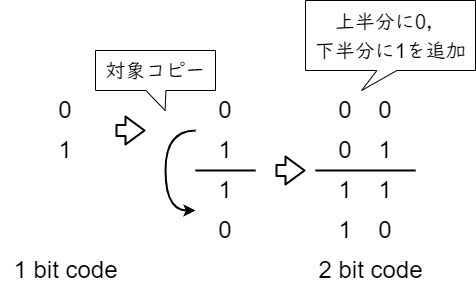
\includegraphics[width=0.4\linewidth]{gray_code.drawio.png}
    \end{center}
\end{defbox}

\begin{table}[htbp]
    \centering
    \caption{10進数の表現}
    \vspace*{-2mm}
    \begin{tabular*}{14.5cm}{wc{2.5cm} wc{2.5cm} wc{2.5cm} wc{2.5cm} wc{2.5cm}} \toprule
        10進数 & 2進数 & BCD & 3増しコード & グレイコード\\ \midrule
        0 & 0000 & 0000 & 0011 & 0000 \\
        1 & 0001 & 0001 & 0100 & 0001 \\
        2 & 0010 & 0010 & 0101 & 0011 \\
        3 & 0011 & 0011 & 0110 & 0010 \\
        4 & 0100 & 0100 & 0111 & 0110 \\
        5 & 0101 & 0101 & 1000 & 0111 \\
        6 & 0110 & 0110 & 1001 & 0101 \\
        7 & 0111 & 0111 & 1010 & 0100 \\
        8 & 1000 & 1000 & 1011 & 1100 \\
        9 & 1001 & 1001 & 1100 & 1101 \\ \bottomrule
    \end{tabular*}
    \label{tab:decimal}
\end{table}

\subsection{負数の表現}

\subsubsection{符号・絶対値表現}

MSBを0なら+,1なら-を表す符号ビットとして用いて,下位のビット列で数の絶対値を表す.
例えば,$-42_{10} = 10101011_2 \ (42_{10} = 00101011_2)$と表現できる.
4ビットの場合の10進数と2進表現の対応を\tref{tab:negative_abs}に示す.

符号なし$n$ビット2進数の場合は,$0$から$2^n-1$までの$2^n$個の数を表現できるが,
符号・絶対値表現を用いた場合はMSBを符号ビットとして用いるため,
$-(2^{n-1} - 1)$から$2^{n-1} - 1$までの$2^{n} - 1$個の数を表現できる.
\tref{tab:negative_abs}から分かるように,$0_{10}$の表現が2つ存在するため,符号なし$n$ビット2進数の場合と比較して表現できる数が1つ少ない.

\begin{table}[htbp]
    \centering
    \caption{符号・絶対値表現}
    \vspace*{-2mm}
    \begin{tabular*}{14cm}{wc{3cm} wc{3cm} wc{3cm} wc{3cm}} \toprule
        10進数 & 2進表現 & 10進数 & 2進表現 \\ \midrule
        -7 & 1111 & +0 & 0000 \\
        -6 & 1110 & +1 & 0001 \\
        -5 & 1101 & +2 & 0010 \\
        -4 & 1100 & +3 & 0011 \\
        -3 & 1011 & +4 & 0100 \\
        -2 & 1010 & +5 & 0101 \\
        -1 & 1001 & +6 & 0110 \\
        -0 & 1000 & +7 & 0111 \\ \bottomrule
    \end{tabular*}
    \label{tab:negative_abs}
\end{table}

\subsubsection{補数}

$n$進数の補数には,$n$の補数と$n-1$の補数が存在する.
それぞれ,以下のように定義されている.

\begin{exprbox}{補数}
    元の数との和が桁上りする数のうち最小のもの.\\
    例1 : $4_{10}$の補数は$6_{10}$ → $4_{10} + 6_{10} = 10_{10}$\\
    例2 : $0011_{2}$の補数は$1101_{2}$ → $0011_{2} + 1101_{2} = 10000_{2}$
\end{exprbox}

\begin{exprbox}{減基数}
    元の数との和が桁上りしない数のうち最大のもの.\\
    例1 : $4_{10}$の補数は$5_{10}$ → $4_{10} + 5_{10} = 9_{10}$\\
    例2 : $0011_{2}$の補数は$1100_{2}$ → $0011_{2} + 1100_{2} = 1111_{2}$
\end{exprbox}

2進数の場合では,2の補数と1の補数が存在する.
1の補数は元の2進数のビット反転で得られ,2の補数は1の補数に1を加えたもので得られる.



\begin{table}[htbp]
    \centering
    \caption{2の補数}
    \vspace*{-2mm}
    \begin{tabular*}{14cm}{wc{3cm} wc{3cm} wc{3cm} wc{3cm}} \toprule
        10進数 & 2進表現 & 10進数 & 2進表現 \\ \midrule
        -8 & 1000 & +0 & 0000 \\
        -7 & 1001 & +1 & 0001 \\
        -6 & 1010 & +2 & 0010 \\
        -5 & 1011 & +3 & 0011 \\
        -4 & 1100 & +4 & 0100 \\
        -3 & 1101 & +5 & 0101 \\
        -2 & 1110 & +6 & 0110 \\
        -1 & 1111 & +7 & 0111 \\ \bottomrule
    \end{tabular*}
    \label{tab:negative_2}
\end{table}

\newpage

\subsection{実数の表現}

\subsubsection{固定小数点表示}

\subsubsection{浮動小数点表示}

\section{演算制御}

\subsection{加減算器}

\subsection{乗算器}

\subsection{除算器}

\subsection{ALU}

\section{アーキテクチャ}

\section{メモリシステム}

\section{オペレーティングシステム}

\subsection{OSの役割}

\begin{enumerate}
    \item ハードウェア機構の隠蔽
    \item ハードウェア装置の管理
    \item ソフトウェア実行時の保護
\end{enumerate}

\section{プロセス管理}

ここで,プロセスとはプログラムとメモリに割り付けられるプロセス領域のことである.
イメージとしては\fref{fig:process}のような,プロセス領域の箱に格納されている任意のプログラムで,プロセス領域が異なれば,プログラムが同じでも別のプロセスとして扱われる.

\fig{0.4}{process.drawio.png}{プロセスのイメージ}{process}

プロセス管理とは,OSによって行われる次のような処理である.

\begin{itemize}
    \item プロセス状態の管理
    \item 実行しているプロセスの切り替え(プロセススイッチ) 
    \item プロセスの生成と消去
    \item プロセス実行順序の決定(プロセススケジューリング)
    \item プロセスからの実行フローの生成と管理
    \item 複数プロセスの同期
    \item 複数プロセス間の通信
\end{itemize}

\subsection{プロセス状態}

プロセスは以下の状態を持ち,\fref{fig:process_state}のように遷移する.

\begin{description}
    \item[実行中 :] プロセッサを占有している状態
    \item[実行可能 :] プロセッサを占有していないが,実行できる状態
    \item[待ち :] プロセッサを占有しておらず,実行できない状態
\end{description}

\fig{0.4}{process_state.drawio.png}{プロセス状態の遷移}{process_state}



\subsection{プロセススケジューリング}

\subsection{プロセス同期}

\subsection{プロセス間通信}



\section{メモリ管理}

\section{入出力制御}

\chapter{離散構造}
集合・命題,関係,漸化式,論理関数,ブール代数,最簡積和形,命題論理,述語論理,導出原理,グラフ

\newpage
\chapter{計算理論}
語・言語,有限オートマトン,正規表現・言語,形式文法とそのクラス,導出・認識・構文解析,文脈自由文法・言語,プッシュダウンオートマトン

\chapter{ネットワーク}
情報源符号化・通信路符号化,階層化モデル,プロトコルとインターフェース,各層プロトコルの設計・仕様・評価手法,ネットワークアプリケーション

\chapter{電子回路と論理設計}
ダイオード・トランジスタ,MOSFET,アナログ電子回路,演算増幅器,記憶素子,数の表現,論理代数と論理関数,組合せ論理回路,順序回路,算術演算回路

\newpage
\chapter{数学解析と信号処理}

\begin{minipage}{0.33\linewidth}
    \begin{itemize}
        \item 微分方程式
        \item フーリエ級数
        \item ラプラス変換
        \item Z変換
    \end{itemize}
\end{minipage}
\hspace{0.05\linewidth}
\begin{minipage}{0.33\linewidth}
    \begin{itemize}
        \item 連続時間信号のフーリエ解析
        \item 離散時間信号のフーリエ解析
        \item 複素関数
    \end{itemize}
\end{minipage}
\hspace{0.05\linewidth}
\begin{minipage}{0.33\linewidth}
    \begin{itemize}
        \item 信号の演算
        \item サンプリング
        \item フィルタ
    \end{itemize}
\end{minipage}

\section{ラプラス変換}\label{sec:laplace_transform}

\begin{defbox}{ラプラス変換}
    $t \ge 0 < \infty$の連続関数$f(t)$について,
    \begin{eqnarray}
        F(s) = \mathcal{L}[f(t)](s) = \int_{0}^{\infty} f(t)e^{-st} dt
        \label{eq:laplace_transform}
    \end{eqnarray}
    が収束するとき,$F(s)$を$f(t)$の\textbf{ラプラス変換}という.
\end{defbox}

\subsection{代表的なラプラス変換}

\begin{exprbox}{指数関数のラプラス変換}
    $s > a$のとき,
    \begin{eqnarray}
        \mathcal{L}[e^{at}](s) = \frac{1}{s - a}
    \end{eqnarray}
    \begin{proof}
        \begin{eqnarray*}
            \mathcal{L}[e^{at}](s) &=& \int_{0}^{\infty} e^{at} e^{-st} dt
            = \lim_{T \to \infty} \int_{0}^{T} e^{-(s - a)t} dt \\
            &=& \lim_{T \to \infty} \left[-\frac{1}{s - a}e^{-(s - a)t}\right]_0^T 
            = \lim_{T \to \infty} -\frac{1}{s - a}e^{-(s - a)T} - \left(-\frac{1}{s - a}\right) \\
            &=& \frac{1}{s - a}
        \end{eqnarray*}
    \end{proof}
\end{exprbox}

\begin{exprbox}{三角関数のラプラス変換}
    $a$を実定数として,
    \begin{eqnarray}
        \mathcal{L}[\cos at](s) = \frac{s}{s^2 + a^2},\hspace{10pt}\mathcal{L}[\sin at](s) = \frac{a}{s^2 + a^2}
    \end{eqnarray}
    \begin{proof}
        $e^{ia} = \cos a + i\sin a$より,
        \begin{eqnarray}
            \cos a = \frac{e^{ia} + e^{-ia}}{2},\hspace{10pt}\sin a = \frac{e^{ia} - e^{-ia}}{2i}
        \end{eqnarray}
        が成り立つ.
        \begin{eqnarray*}
            \mathcal{L}[\cos at](s) &=& \mathcal{L}[\frac{e^{iat} + e^{-iat}}{2}](s)
            = \frac{1}{2}\left(\mathcal{L}[e^{iat}](s) + \mathcal{L}[e^{-iat}](s)\right)\\
            &=& \frac{1}{2} \left(\frac{1}{s - ia} + \frac{1}{s + ia}\right)
            = \frac{1}{2} \frac{2s}{s^2 - (ia)^2} \\
            &=& \frac{s}{s^2 + a^2}
        \end{eqnarray*}
        同様に
        \begin{eqnarray*}
            \mathcal{L}[\sin at](s) &=& \mathcal{L}[\frac{e^{iat} - e^{-iat}}{2i}](s)
            = \frac{1}{2i}\left(\mathcal{L}[e^{iat}](s) - \mathcal{L}[e^{-iat}](s)\right)\\
            &=& \frac{1}{2i} \left(\frac{1}{s - ia} - \frac{1}{s + ia}\right)
            = \frac{1}{2i} \frac{2ia}{s^2 - (ia)^2} \\
            &=& \frac{a}{s^2 + a^2}
        \end{eqnarray*}
    \end{proof}
\end{exprbox}

\begin{exprbox}{双曲線関数のラプラス変換}
    $a$を実定数として,
    \begin{eqnarray}
        \mathcal{L}[\cosh at](s) = \frac{s}{s^2 - a^2},\hspace{10pt}\mathcal{L}[\sinh at](s) = \frac{a}{s^2 - a^2}
    \end{eqnarray}
    \begin{proof}
        双曲線関数を以下のように定義する.
        \begin{eqnarray}
            \cosh a = \frac{e^{a} + e^{-a}}{2},\hspace{10pt}\sinh a = \frac{e^{a} - e^{-a}}{2}
        \end{eqnarray}
        \begin{eqnarray*}
            \mathcal{L}[\cosh at](s) &=& \mathcal{L}[\frac{e^{at} + e^{-at}}{2}](s)
            = \frac{1}{2}\left(\mathcal{L}[e^{at}](s) + \mathcal{L}[e^{-at}](s)\right)\\
            &=& \frac{1}{2} \left(\frac{1}{s - a} + \frac{1}{s + a}\right)
            = \frac{1}{2} \frac{2s}{s^2 - a^2} \\
            &=& \frac{s}{s^2 - a^2}
        \end{eqnarray*}
        同様に
        \begin{eqnarray*}
            \mathcal{L}[\sinh at](s) &=& \mathcal{L}[\frac{e^{at} - e^{-at}}{2}](s)
            = \frac{1}{2}\left(\mathcal{L}[e^{at}](s) - \mathcal{L}[e^{-at}](s)\right)\\
            &=& \frac{1}{2} \left(\frac{1}{s - a} - \frac{1}{s + a}\right)
            = \frac{1}{2} \frac{2a}{s^2 - a^2} \\
            &=& \frac{a}{s^2 - a^2}
        \end{eqnarray*}
    \end{proof}
\end{exprbox}

\begin{exprbox}{多項式のラプラス変換}
    \begin{eqnarray}
        \mathcal{L}[t^n](s) = \frac{n!}{s^{n + 1}}
    \end{eqnarray}
    \begin{proof}
        $F_n(s) = \mathcal{L}[t^n](s)$と定義して,
        \begin{eqnarray*}
            F_n(s) &=& \int_{0}^{\infty} t^n e^{-st} dt
            = \left[t^n \left(-\frac{1}{s} e^{-st}\right)\right]_0^\infty - \int_{0}^{\infty} n t^{n - 1} \left(-\frac{1}{s} e^{-st}\right) dt \\
            &=& \frac{n}{s} \int_{0}^{\infty} t^{n - 1} e^{-st} dt = \frac{n}{s} \mathcal{L}[t^{n - 1}](s)
            = \frac{n}{s} F_{n - 1}(s) \\
            &=& \frac{n}{s} \frac{n - 1}{s} \cdots \frac{1}{s} F_0(s) \\
            F_0(s) &=& \mathcal{L}[t^0](s) = \int_{0}^{\infty} e^{-st} dt \\
            &=& \left[-\frac{1}{s}e^{-st}\right]_0^\infty = \frac{1}{s} \\
            \therefore F_n(s) &=& \frac{n!}{s^{n + 1}}
        \end{eqnarray*}
    \end{proof}
\end{exprbox}

\newpage

\subsection{ラプラス変換の性質}

\begin{exprbox}{線形性}
    連続関数f(t),g(t)がラプラス変換可能なら,次が成り立つ.
    \begin{eqnarray}
        \mathcal{L}[a f(t) + b g(t)](s) = a\mathcal{L}[f(t)](s) + b\mathcal{L}[g(t)](s)
    \end{eqnarray}
    \begin{proof}
        \begin{eqnarray*}
            \mathcal{L}[a f(t) + b g(t)](s) &=& 
            \int_{0}^{\infty} \left(a f(t) + b g(t)\right) e^{-st} dt\\
            &=& a \int_{0}^{\infty} f(t) e^{-st} dt + b \int_{0}^{\infty} g(t) e^{-st} dt \\
            &=& a\mathcal{L}[f(t)](s) + b\mathcal{L}[g(t)](s)
        \end{eqnarray*}
    \end{proof}
\end{exprbox}

\begin{exprbox}{像の移動法則}
    \begin{eqnarray}
        \mathcal{L}[e^{at}f(t)](s) = F(s - a)
    \end{eqnarray}
    \begin{proof}
        \begin{eqnarray*}
            \mathcal{L}[e^{at}f(t)](s) &=& \int_{0}^{\infty} e^{at} f(t) e^{-st} dt
            = \int_{0}^{\infty} f(t) e^{-(s - a)t} dt \\
            &=& \mathcal{L}[f(t)](s - a) = F(s - a)
        \end{eqnarray*}
    \end{proof}
\end{exprbox}

\begin{exprbox}{微分法則}
    \begin{eqnarray}
        \mathcal{L}[f'(t)](s) &=& sF(s) - f(0) \\
        \mathcal{L}[f''(t)](s) &=& s^2F(s) - sf(0) - f'(0) \\
        \vdots \\
        \mathcal{L}[f^{(n)}(t)](s) &=& s^nF(s) - s^{n - 1}f(0) - s^{n - 2}f'(0) - \cdots - f^{(n)}(s)
    \end{eqnarray}
    \begin{proof}
        \begin{eqnarray*}
            \mathcal{L}[f'(t)](s) &=& \int_{0}^{\infty} f'(t) e^{-st} dt
            = \left[f(t) e^{-st}\right]_0^\infty - \int_{0}^{\infty} f(t) se^{-st} dt
            = -f(0) + s \int_{0}^{\infty} f(t) e^{-st} dt\\
            &=& sF(s) - f(0)
        \end{eqnarray*}
        \begin{eqnarray*}
            \mathcal{L}[f''(t)](s) &=& \mathcal{L}[\left(f'(t)\right)'](s) \\
            &=& s \mathcal{L}[f'(t)](s) - f'(0) = s\left(sF(s) - f(0)\right) - f'(0) \\
            &=& s^2 F(s) - s f(0) - f'(0)
        \end{eqnarray*}
        同様に
        \begin{eqnarray*}
            \mathcal{L}[f^{(n)}(t)](s) &=& s^nF(s) - s^{n - 1}f(0) - s^{n - 2}f'(0) - \cdots - f^{(n)}(s)
        \end{eqnarray*}
    \end{proof}
\end{exprbox}

\begin{exprbox}{像の微分法則}
    \begin{eqnarray}
        \mathcal{L}[t f(t)](s) = -\frac{d}{ds} F(s),\hspace{10pt}\mathcal{L}[t^n f(t)] = \left(-\frac{d}{ds}\right)^n F(s)
        \label{eq:laplace_image_derivative}
    \end{eqnarray}
    \begin{proof}
        $F_n(s) = \left(-\frac{d}{ds}\right)^n F_0(s)$として,
        \begin{eqnarray*}
            F_1(s) &=& -\frac{d}{ds}F_0(s) = \int_{0}^{\infty} -\frac{\partial}{\partial s} \left\{e^{-st} f(t)\right\} dt
            = \int_{0}^{\infty} t f(t) e^{-st} dt = \mathcal{L}[tf(t)](s) \\
            F_2(s) &=& \left(-\frac{d}{ds}\right) F_1(s) 
            = \int_{0}^{\infty} -\frac{\partial}{\partial s} \left\{t f(t) e^{-st}\right\} dt
            = \int_{0}^{\infty} t^2 f(t) e^{-st} dt = \mathcal{L}[t^2f(t)](s)
        \end{eqnarray*}
        同様に
        \begin{eqnarray*}
            F_n(s) = \mathcal{L}[t^nf(t)](s)
        \end{eqnarray*}
    \end{proof}
\end{exprbox}

\begin{exprbox}{相似法則}
    \begin{eqnarray}
        \mathcal{L}[f(at)](s) = \frac{1}{a}F\left(\frac{s}{a}\right)
    \end{eqnarray}
    \begin{proof}
        \begin{eqnarray*}
            \mathcal{L}[f(at)](s) = \int_{0}^{\infty} f(at) e^{-st} dt
            \overset{u = at}{=} \int_{0}^{\infty} f(u) e^{-\frac{s}{a}u} \frac{dt}{a}
            = \frac{1}{a} F\left(\frac{s}{a}\right)
        \end{eqnarray*}
    \end{proof}
\end{exprbox}

\begin{exprbox}{たたみ込み}
    畳み込みを次の式で定義する.
    \begin{eqnarray}
        f \ast g(t) = \int_{0}^{t} f(\tau)g(t - \tau) d\tau
    \end{eqnarray}
    このとき,畳み込みのラプラス変換は次のようにラプラス変換の積となる.
    \begin{eqnarray}
        \mathcal{L}[f \ast g(t)](s) = F(s)G(s)
    \end{eqnarray}
    \begin{proof}
        \begin{eqnarray*}
            F(s)G(s) &=& G(s) \int_{0}^{\infty} f(\tau) e^{-s\tau} d\tau
            = \int_{0}^{\infty} f(\tau) G(s) e^{-s\tau} d\tau
        \end{eqnarray*}
        ここで,
        \begin{eqnarray*}
            G(s) e^{-s\tau} &=& \int_{0}^{\infty} e^{-sx} g(x) dx e^{-s\tau}
            = \int_{0}^{\infty} g(x) e^{-s(x+\tau)} dx \\
            &\overset{t = x + \tau}{=}& \int_{\tau}^{\infty} g(t - \tau) e^{-st} dt
        \end{eqnarray*}
        なので,もとの式に代入して,
        \begin{eqnarray*}
            F(s)G(s) &=& \int_{0}^{\infty} f(\tau) \left\{\int_{\tau}^{\infty} g(t - \tau) e^{-st} dt\right\} d\tau
        \end{eqnarray*}
        領域$D: t \ge \tau, \tau \ge 0$は領域$D': 0 \le \tau \le t, t \ge 0$と等しいため,次のようになる.
        \begin{eqnarray*}
            F(s)G(s) &=& \int_{0}^{\infty} \int_{0}^{t} f(\tau) g(t - \tau) e^{-st} d\tau dt\\
            &=& \int_{0}^{\infty} \left\{\int_{0}^{t} f(\tau) g(t - \tau) d\tau\right\} dt
            = \mathcal{L}[f \ast g(t)](s)
        \end{eqnarray*}
    \end{proof}
\end{exprbox}

\subsection{ラプラス変換表}

\begin{minipage}{0.5\linewidth}
    \centering
    \begin{tabular*}{6.88cm}{wc{3cm}wc{3cm}} \toprule
        $1$ & $\frac{1}{s}$ \\ 
        $t^n$ & $\frac{n!}{s^{n+1}}$ \\
        $t^\alpha$ & $\frac{\Gamma(\alpha + 1)}{s^{\alpha+1}}$ \\\bottomrule
    \end{tabular*}
\end{minipage}
\begin{minipage}{0.5\linewidth}
    \begin{tabular*}{6.88cm}{wc{3cm}wc{3cm}} \toprule
        $1$ & $\frac{1}{s}$ \\ \bottomrule
    \end{tabular*}
\end{minipage}

\subsection{ラプラス変換が存在する条件}

\subsection{ラプラス変換の応用}

\subsubsection{特殊な積分}

ラプラス変換を用いることで,いくつかの特殊な積分を簡単に解ける.
以下に例を示す.

\begin{exprbox}{ディリクレ積分}
    \begin{eqnarray}
        \int_{0}^{\infty} \frac{\sin t}{t} dt = \frac{\pi}{2}
    \end{eqnarray}
    \begin{proof}
        \begin{eqnarray*}
            J(s) = \mathcal{L}\left[\frac{\sin t}{t}\right] = \int_{0}^{\infty} \frac{\sin t}{t} e^{-st} dt
        \end{eqnarray*}
        と定義する.像の微分法則(\eref{eq:laplace_image_derivative})より,
        \begin{eqnarray*}
            \frac{dJ}{ds}(s) = - \mathcal{L}\left[t \frac{\sin t}{t}\right](s) = -\mathcal{L}[\sin t](s) = - \frac{1}{s^2 + 1}
        \end{eqnarray*}
        となるので,任意定数$C$について次の式が成り立つ.
        \begin{eqnarray*}
            J(s) = -\arcsin s + C
        \end{eqnarray*}
        $\lim_{s \to \infty} J(s) = 0$,$\lim_{s \to \infty} = \frac{\pi}{2}$より,$C = \frac{\pi}{2}$である.
        したがって,$J(0) = \frac{\pi}{2}$より,
        \begin{eqnarray*}
            \int_{0}^{\infty} \frac{\sin t}{t} dt = \frac{\pi}{2}
        \end{eqnarray*}
    \end{proof}
\end{exprbox}

\subsubsection{常微分方程式}

\subsection{まとめ}

\section{z変換}\label{sec:z_transform}

\section{フーリエ変換}\label{sec:fourier_transform}

\section{変換表}

\end{document}